\section{System Overview (75 pts)\label{sec:1}}

    \begin{figure}
        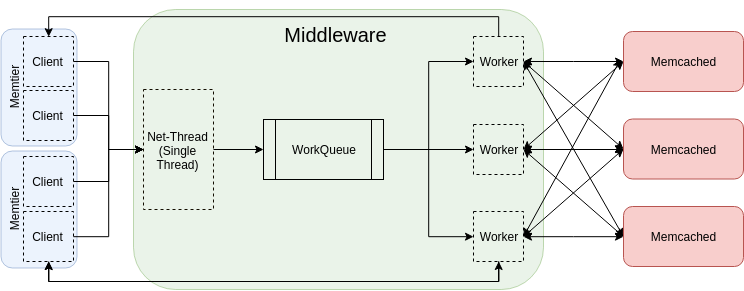
\includegraphics[width=0.8\linewidth]{graphics/system-request-flow.png}
        \caption{Basic flow of information in the system. Each box with a dashed border indicates a thread on the
                 respective system which are colour coded into 3 categories, blue for \cli, green for \mw{} and red for
                 \srv. Arrows denote the order of flow of information.\label{fig:request-overview}}
    \end{figure}

    The abstract flow of requests through the system is visualized in figure \ref{fig:request-overview}. The lifetime
    of a request begins in a thread on memtier, is received by the Net-Thread and upon receiving a complete packet
    it is stored in the WorkQueue. This queue is shared for any threads in the middleware and they compete for each
    individual element. The moment a Worker receives the request it processes it locally, checks the type and first
    sends the request to either one connected memcached (non-sharded GET) or all connected memcached instances
    (sharded GET and SET). Upon receiving replies from memcached there are checks for what was received and sanity
    checks included (e.g. receiving a SET reply for a GET reply is clearly an ERROR) before sending back a constructed
    reply directly from the worker thread to memtier given enough replies have been received. As such the Middleware
    receives only via the Net-Thread and only sends only via the worker when communicating with memtier instances.
    Communication between memcached follows a client-server model, the middleware being the client.

    \subsubsection{System Component Overview}
        For network communication Java NIO is used for all connections. The Net-Thread uses a \tw{ServerSocketChannel}
        whereas worker threads employ for each connection with memcached an instance-private \tw{SocketChannel}, all
        connections configured to be non-blocking. With the use of Java NIO \tw{Channel}s writes are expected to perform
        more ideal in distribution from the middleware to either memcached or memtier. To manage connections the
        Net-Thread employs a single \tw{Selector} which handles memtier connections, each worker thread two\textemdash
        one to manage all memcached connections and another to interact with memtier using referenced \tw{SelectionKey}s
        from the Net-Thread's Selector. To allow handling of multiple requests the Net-Thread spawns a fixed amount of
        worker threads once at the start, all attached to an \tw{ExecutorService} and upon finishing return gathered
        thread statistics. This is achieved by worker threads implementing the \tw{Callable} interface. The gathered
        statistics are to be saved by the net-thread for each finished worker before termination. Termination can be
        achieved by sending the middleware a \tw{SIGTERM} signal; a shutdown hook is installed right after the
        middleware is instantiated by the given wrapper class.\newline
        For the WorkQueue depicted an \tw{ArrayBlockingQueue} is used, meaning blocking behaviour can be expected for
        the Net-Thread if the queue fills up with requests and blocking behaviour for workers should not enough requests
        exist. As such, the only producer is the Net-Thread and the only consumers worker threads. The content of the
        WorkQueue are \tw{WorkUnit}s which are interpreted requests/replies and designed to be more programmer friendly
        than simple \tw{byte[]}-arrays at the expense of more garbage collection. These WorkUnits are the result of
        successfully receiving data from either party and the product of a \tw{PacketParser}, used by connections of the
        Net-Thread and worker threads. It is designed in a stateful approach and as such each connection has a logically
        private instance of a PacketParser attached to it. This binding is done after the first successful registration
        of new connections.

    \subsubsection{Request Handling}
        Before any requests are processed by the middleware any incoming memtier connections must be first
        \tw{accept()}-ed by the Net-Thread and registered in the attached Selector. Once done the PacketParser is called
        each time the OS notifies of new data being available on a registered SelectionKey. The PacketParser is designed
        to read data from a socket into a directly allocated \tw{ByteBuffer} (size = \SI{8192}{\byte}), generate a
        timestamp for the call to read data from the socket, receive data from the socket, parse the received data and
        extract at most a single request/reply, compact the ByteBuffer and store the result on success. This process is
        repeated as long as a request is stored (\textrightarrow{} returns a \tw{List} of WorkUnit) and as such follows a
        greedy approach. The design aims to fully exhaust the data received from a single client before parsing new
        data. This would be troublesome in the general case of long streams but this is not expected and aims to allow
        quicker handling of single requests once they get actively processed. In the process of extracting data, three
        basic steps are done: read the current stream of Bytes linearly until \tw{"\textbackslash r\textbackslash n"} is
        encountered, extract the data and match it Byte-by-Byte to a list of supported headers and extract type-specific
        header fields as per memcached documentation, and lastly either return the result as no body is expected or try
        to get the rest of the body. The body is read in a single command as is therefore likely to need multiple
        repetitions as MTUs are limited to \SI{1500}{\byte} but the body being \SI{4096}{\byte}. As such internal
        state is kept over rounds as to what part of a packet is currently expected to be processed. Once enough data is
        buffered the data is then copied and the result returned. As previously noted this result is a \tw{WorkUnit}. It
        holds next to the received header and body (as \tw{byte[]}) also fields for the type, type-specific fields (such
        as the list of keys for GET requests), the SelectionKey from which it was received and also a timestamp-object
        which keeps track on statistics when a packet was received (the moment of calling to parse incoming data),
        enqueued into the WorkQueue, dequeued from it, when it was ready to be sent to memcached, when all replies were
        received for it from memcached and finally when the reply was sent back to memtier.\newline
        The PacketParser returns once all data was consumed and returns a list of received packets. These are then
        stored to the WorkQueue for worker threads to process.

        Processing WorkUnits on a worker follows the outline of dequeueing an element, checking its type, sending the
        request to either one (non-sharded GET) or all/some connected memcached servers (sharded multi-key GET or SET),
        waiting for the appropriate amount of replies, doing some local processing of the replies, sending it to the
        WorkUnit's attached SelectionKey and then dequeue another element, thus restarting the loop. Upon dequeueing the
        element is checked to be of type GET, SET, an invalid packet or anything else (the latter two resulting in
        logged messages). For SET requests the worker thread prepares for each memcached-instance connected to, a new
        ByteBuffer with a copy of the request and sends it to all memcached servers. It waits for each server to reply
        with 3 messages and verifies the content to be only STORED. On a failure an error message is returned, on a
        match any of the three requests chosen and sent back to the recipient by dereferencing the associated
        SocketChannel with the original WorkUnit. GET requests are prepared with load-balancing
        schemes (described in thorough detail later) depending on enabling or disabling sharding. The amount of keys in
        each GET (GETs with keys\,>\,1 are called \emph{multi-GET}) is of minor significance of load balancing. For the
        non-sharded case a single packet (a ByteBuffer) is created, the size remembered for load-balancing purposes and
        mapped to the server with the smallest load. For the sharded case mappings of packets to servers in the degree
        of distributed load are generated. Skewed loads result in the degenerated case of a non-sharded multi-GET, good
        cases in a fair distribution of requests to servers (logically, they have not yet been sent, only prepared).
        After the packets are created and mapped to servers an expectation of replies is set for each memcached instance
        and the routine referenced in the distribution of SET requests is called. It is universal enough to also deal
        with misses and stops listening to the memcached instance once an ``END'' is received and internal state
        updated. After receiving all necessary replies sanity checks are again made, received ``VALUE'' requests
        serialized and an ``END'' packet appended to the collection of packets before a ByteBuffer is created from the
        replies and then sent to the respective memtier instance. In all cases where replies are received from memcached
        the associated PacketParser is used to read the received data and resulting WorkUnits stored in a result list.
        These WorkUnits are only processed to infer the validity of the replies from memcached.

    \subsubsection{System Instrumentation}
        For the following events in the system performance benchmark results are generated: In the PacketParser on the
        relating call when a header is correctly parsed (\textrightarrow{} timestamp for package arrived in the system,
        stored in the respective WorkUnit), on an enqueue and dequeue to the WorkQueue (\textrightarrow{} the current
        queue size is logged after the operation completed successfully, the only statistic on the Queue; additionally
        in both cases the WorkUnit gets the timestamp logged for the respective event) and at the following points in
        the worker thread. The aforementioned dequeue also generates packet-type specific metrics. For all valid types
        (SET, GET and multi-GET) the count of observed elements is incremented and the time on the queue logged. GETs of
        multiple keys also log the amount of keys. For invalid packets a counter is incremented. Before communication
        with memcached occurs but after the keys have already been mapped for servers and packets created a timestamp is
        stored in the WorkUnit. In case of an unexpected amount of GET replies the number of missing keys is logged for
        GET requests disregarding their size. It is still possible to infer whether the reason was a single-key or a
        multi-key GET. Another timestamp is generated after receiving and having processed all request-related replies
        as well in the WorkUnit (marks stop of memcached communication). In addition to this timestamp the communication
        with memcached and packet processing is logged for the respective request type. A last timestamp is stored the
        moment the reply has been successfully written to memtier's SocketChannel. This again also incurs a store of the
        total duration the WorkItem has been in the system and simulates an RTT through the system in addition to
        generating a statistic used for creating histograms (with \SI{100}{\micro\second} precision). Lastly at
        termination of the each worker thread the observed load distribution is remembered. All datapoints captured by a
        worker are upon termination accumulated and averaged (where applicable) in relation to the percentage of
        requests they served.\newline
        Timestamps on WorkItems are used to populate the aforementioned type-specific request metrics. All metrics
        mentioned that are not timestamps are accumulated in 1 second windows and in all cases but the load distribution
        and counters for requests / cache misses are averaged by the number of observed datapoints. This averaging is a
        simple arithmetic mean. The metrics on cache misses and request counts are simple counts and not averaged. The
        load distribution is continuously updated but returns an overall view at the end of the lifetime of the thread.

        To start logging a common timestamp is set once the first packet has been fully parsed and ready to be dequeued.
        A final timestamp is set in the Net-Thread after all worker threads have finished execution.

    \subsubsection{Load Balancing GET requests}
        % Load balancing of requests to memcached instances is only explicitly done for GET requests (SET requests must be
        % distributed to all memcached instances anyways).
        Each worker thread remembers which memcached instance received how much load and tries to balance requests based
        on the key-size passed and whether sharding is enabled or not.  For non-sharded behaviour the best effort that
        can be done is returning always the memcached instance with the lowest amount of requests sent. On a tie any of
        the valid candidates is fine to be selected. For sharded requests this idea is further refined by the use of a
        sorting network which gives access to the memcached instances in an ordered approach. There the server with the
        smallest amount of work is greedily chosen and given as many keys as are required to close the gap to the second
        lowest server. This leads to either exhaustion of requests and one memcached instance is put under load or keys
        still need to be distributed amongst memcached instances. In this case two servers now exist with equal amounts
        of smallest load and another, new second lowest server must be found. Again keys are distributed equally such
        that the first two servers have now at least the load of the third server. As the experiments don't use more
        than three servers any leftover keys are distributed in an even fashion amongst memcached instances. Any uneven
        distributions for one multi-key GET request will be evened out by future ones as servers with high load are
        deprioritized with this algorithm. It is not required that worker threads communicate the amount of load each
        memcached server was subject to as on average this design converges towards a fair estimate of equal load being
        distributed to all participants.


    \subsection{Experimental Configurations\label{subsec:1_exp-conf}}
        In this report the following notations exist: \cli, \mw{} and \srv{} which refer
        to instances of virtual machines on Microsoft Azure of the following configurations.

        Basic A1 (1\,vcpu, \SI{1.75}{\giga\byte} RAM) are used for \srv{} actors, Basic A2 (2vcpu, \SI{3.5}{\giga\byte}
        RAM) for \cli{} actors and lastly Basic A4 (8vcpu, \SI{14}{\giga\byte} RAM) for \mw{} actors. All instances are
        running Ubuntu 16.04.5 LTS. Instance specific configurations for the experiments are the following:

        \begin{table}
            \footnotesize{
            \centering
            \captionsetup{justification=centering}
            \ra{1.1}
            \begin{tabular}{@{}rlllll@{}}
                    \toprule
                    \textbf{Machine Type} & \textbf{Throughput [Mbit/s]} & \textbf{SET request} &
                    \textbf{SET reply} & \textbf{GET request} & \textbf{GET reply} \\
                    \midrule
                    \cli & 201 & 6077.65     & \textemdash   & $1.32 * 10^6$ & \textemdash \\
                    \mw  & 802 & 24267.73    & $2.25 * 10^7$ & $5.27 * 10^6$ & 24261.85 \\
                    \srv & 101 & \textemdash & $1.57 * 10^6$ & \textemdash   & 3055.42 \\
                    \bottomrule
            \end{tabular}
            \caption{Derived maximal requests per second for given upload speeds. Maximum request numbers per
                     seconds are based on sizes of \SI{4131}{\byte}, \SI{8}{\byte}, \SI{19}{\byte} and \SI{4132}{\byte}
                     for SET requests, SET replies, GET requests and GET replies respectively. These calculations
                     exclude any network overhead.\label{tab:iperf_results}}
            }
        \end{table}

        \begin{enumerate}
            \item \cli{}s run memtier 1.2.15 %\footnote{\url{https://github.com/RedisLabs/memtier_benchmark}} 1.2.15
                  to generate load on the system.
                  The memtier configuration is the most variable over the run of experiments. As a basic building
                  block the following command line is used for non-multiget request:
                  \tw{memtier -\/-protocol=memcache\_text -\/-expiry-range=259200-259201
                      -\/-key-maximum=10000 -\/-data-size=4096 \newline
                      -\/-clients=\$VIRTUAL\_CLIENTS -\/-threads=\$THREADS
                      -\/-test-time=\$RUNTIME \newline -\/-server=\$REMOTE
                      -\/-port=\$PORT -\/-ratio=\$SET\_RATIO:\$GET\_RATIO}

                  For multiget requests the \tw{-\/-ratio} parameter reads in the size of the requested multiget
                  size and also adds the argument \tw{-\/-multi-key-get=\$MULTIGET\_COUNT}. These variables are set
                  according to experimental paramters.

            \item \mw{}s use OpenJDK 8 to run the middleware software.
                  The middleware accepts as input parameters the number of threads, whether sharding is to be used
                  for MultiGET requests and the memcached instances to connect to. The experiments describe the
                  respective invocations of the middleware. As a basic building block the following command line is
                  used:
                  \tw{java -jar \$JAR\_PATH -l \$LISTEN\_IP -p \$LISTEN\_PORT -t \$WORKER\_THREADS -s \$IS\_SHARDED
                      -m \$SERVER\_PORT\_PAIR[*]}

                   The last parameter is the list of memcached server IPs with ports to connect to.

            \item \srv{}s run memcached 1.4.25 to reply to requests sent by memtier.
                  The memcached configuration was configured to listen on any incoming requests with a single thread
                  (\tw{-l 0.0.0.0 -t 1}) and started as a system service.

            \item All machines further use dstat to log resource usage in general next to pings between interacting
                  machines. Additionally iperf statistics were generated between each client type to show network
                  limits for upload and download speeds. A tabularized summary can be found in table
                  \ref{tab:iperf_results}.
        \end{enumerate}

        The key size for the experiments has been fixed to \SI{4096}{\byte}, the maximal key index to 10000 and their
        lifetime set to \SI{259200}{\second} (\SI{72}{\hour}) to prevent misses. Before experiments were conducted
        each \srv{}'s memcached instance was populated with dummy values using the following command:
        \tw{memtier -\/-protocol=memcache\_text -\/-expiry-range=259200-259201 -\/-key-maximum=10000 -\/-data-size=4096
            -\/-clients=1 -\/-threads=2 -\/-requests=10001 \newline -\/-ratio=1:0 -\/-key-pattern=S:S
            -\/-server=\$REMOTE -\/-port=\$PORT}

        Using the included wrapper of memtier which automatically infers the amount of keys used resulted in misses,
        likely due to a fencepost error in key calculations internally.

        Experimental results were gathered for sets of runs. Experimental data was gathered for experiment 2 in a
        single run, for experiment 3 in a single run and experiments 4\textendash6 were gathered in one single run
        together (Best effort approaches were made to run everything in one run yet due to financial reasons and
        Microsoft Azure's cloud being a turbulent environment single experiments with insufficiently comparable data
        needed to be run multiple times.) Each configuration was tested for \SI{80}{\second} three times with a stable
        window of \SI{60}{\second} being cut from the logs after \SI{10}{\second} have elapsed.

        A note on statistics. During the analysis is has been inferred that queue sizes were not matching with the
        per-thread queue waiting time statistics gathered. For small loads a generally too high queue size was predicted
        whereas for high loads too small. The queue waiting times are in their design of the middleware a much better
        indicator of the queue size and as such the queue size reported is directly derived by the throughput for the
        window multiplied by the queue waiting time in this report (normalized to \SI{1}{\second}. The reason for
        incorrect queue sizes inferred by the middleware is due to an imprecise locking approach on statistics
        gathering.

        All graphs except histograms, residual plots and QQ plots error have bands/bars given in this report.
